%!TEX options = -shell-escape

\documentclass[12pt]{report}
\usepackage[a4paper,twoside,top=20mm,bottom=20mm,inner=30mm,outer=25mm]{geometry}
\usepackage[utf8]{inputenc}
\usepackage[greek,english]{babel}
\usepackage[scaled=0.86]{couriers}
\usepackage[toc,page,title,titletoc]{appendix}
\usepackage[pdfpagelabels,unicode]{hyperref}
\usepackage{bookmark}
\usepackage[fixlanguage]{babelbib}
\selectbiblanguage{greek}
\usepackage{titlesec}
\usepackage{etoolbox}
\usepackage{graphicx}
\usepackage{array}
\usepackage{amsmath}
\usepackage{minted}
\usepackage{subcaption}
\captionsetup{compatibility=false}
\graphicspath{ {images/} }
\usepackage[noend]{algpseudocode}
\usepackage{algorithm}
\usepackage{afterpage}
\usepackage{comment}
\usepackage{float}
\usepackage{listings}
\lstset{language=sh,
        showstringspaces=false,
        basicstyle=\ttfamily\footnotesize,
        breaklines=true}

\newcommand\blankpage{%
    \null
    \thispagestyle{empty}%
    \addtocounter{page}{-1}%
    \newpage}

\hypersetup{
  colorlinks=true,
  % linkcolor=green,
  citecolor=red,
  % filecolor=blue,
  urlcolor=blue,
  % pdftitle=,
  % pdfauthor=,
  % pdfsubject=,
  % pdfkeywords=
}

\setcounter{secnumdepth}{3}
\setcounter{tocdepth}{3}

\titleformat{\chapter}
  {\normalfont\LARGE\bfseries}{\thechapter}{1em}{}
\titlespacing*{\chapter}{0pt}{3.5ex plus 1ex minus .2ex}{2.3ex plus .2ex}

\makeatletter
\patchcmd\@resets@pp{%
  \def\Hy@chapapp{\appendixname }%
}{%
  \def\Hy@chapapp{appendix}%
}{}{\errmessage{Cannot patch \string\@resets@pp}}
\patchcmd\@resets@ppsub{%
  \def\Hy@chapapp{\appendixname }%
}{%
  \def\Hy@chapapp{appendix}%
}{}{\errmessage{Cannot patch \string\@resets@pp}}
\makeatother

\addto{\captionsgreek}{\renewcommand{\appendixpagename}{Παραρτήματα}}
\addto{\captionsgreek}{\renewcommand{\appendixtocname}{Παραρτήματα}}
\addto{\captionsgreek}{\renewcommand{\appendixname}{Παράρτημα}}

\begin{document}
\selectlanguage{greek}

\hypersetup{pageanchor=false}

\begin{titlepage}
  \centering
  
\includegraphics[width=0.15\textwidth]{pyrforos}\par\vspace{1cm}
  {\scshape\LARGE Εθνικό Μετσόβιο Πολυτεχνείο\\
  Σχολή Ηλεκτρολόγων Μηχανικών και Μηχανικών Η/Υ\par}
  \vspace{1cm}
  {\scshape\Large Εργασία στο Μεταπτυχιακό Μάθημα\\
  Πολυμεσικό Υλικό στο Internet: Συγχρονισμός, Επεξεργασία και Διακίνηση\par}
  \vspace{1.5cm}
  {\Large\bfseries Εγκατάσταση του \textlatin{Open edX} και Δημιουργία Ενδεικτικού Ιστοτόπου Μαθήματος (\textlatin{Microsite})\par}
  \vspace{2cm}
  {\large Δημήτριος Πολίτης (ΥΔ)\par}
  \vfill
  Επιβλέπων \par
  Καθ. Ευστάθιος Συκάς

  \vfill

% Bottom of the page
  {\large \today\par}
  \afterpage{\blankpage}
\end{titlepage}

\tableofcontents
\thispagestyle{empty}

\listoffigures
\thispagestyle{empty}

\begin{abstract}
Στο παρόν παρουσιάζεται η λειτουργία και η διαδικασία ανάπτυξης ενός μαθήματος στην πλατφόρμα \textlatin{Open-EDX}. Αρχικά  γίνεται αναφορά στην εν λόγω πλατφόρμα ηλεκτρονικής μάθησης και στη συνέχεια περιγράφεται αναλυτικά η διαδικασία εγκατάστασης της, με τη χρήση αυτοματοποιημένων εργαλείων (\textlatin{ansible, vagrant}). Τέλος περιγράφεται ο τρόπος δημιουργίας εντός τής πλατφόρμας, ενός ενδεικτικού ιστοτόπου μαθήματος. Η εργασία είναι διαθέσιμη από το σύνδεσμο \textlatin{\url{https://github.com/dpolitis/open-edx-install}}.

\vspace{10mm}

\noindent \textbf{Λέξεις κλειδιά:} Ηλεκτρονική Μάθηση, Ανοιχτός Κώδικας, Διαδίκτυο.
\end{abstract}

\hypersetup{pageanchor=true}
\clearpage
\pagenumbering{arabic}

\chapter{Εισαγωγή}\label{ch1}
\section{Εισαγωγή}
Η εποχή του Διαδικτύου επιβάλει την αναθεώρηση των παραδοσιακών τρόπων διεξαγωγής της διδασκαλίας μέσω φυσικής επαφής. Πλέον μεγάλο ποσοστό των μαθημάτων στην ακαδημαϊκή κοινότητα, πραγματοποιούνται με ηλεκτρονικά μέσα.

Η δημιουργία, η συντήρηση και η ανανέωση του περιεχομένου στις πλατφόρμες ηλεκτρονικής μαθησης αποτελεί σημαντικό παράγοντα στον κύκλο της μάθησης. Πλέον οι πλατφόρμες αυτές δεν περιορίζονται στην παροχή ηλεκτρονικών εγχειριδίων και σημειώσεων, αλλά αποτελούν πλέον εικονικές αίθουσες διδασκαλίας με τις δυνατότητες χρήσης \textlatin{live video streaming} ή \textlatin{avatar}.

\section{Ηλεκτρονική Μάθηση}
\subsection{Ορισμοί - Έννοιες}
Ηλεκτρονική Μάθηση ορίζεται ως η χρήση ηλεκτρονικών μέσων, εκπαιδευτικών τεχνολογιών αλλά και τεχνολογιών πληροφορίας και επικοινωνίας (ΤΠΕ) στην εκπαίδευση~\cite{wikipedia_2018_1}. Η ηλεκτρονική μάθηση διακρίνεται επιμέρους στη Σύγχρονη και Ασύγχρονη μάθηση.
  \paragraph{Σύγχρονη Mάθηση.} Ο όρος σύγχρονη μάθηση χρησιμοποιείται για να περιγράψει μορφές μάθησης και διδασκαλίας που λαμβάνουν χώρα την ίδια χρονική στιγμή, αλλά όχι στον ίδιο χώρο. Η Σύγχρονη μάθηση απαιτεί την ταυτόχρονη συμμετοχή του εκπαιδευτή και του εκπαιδευόμενου, όπου η αλληλεπίδραση μεταξύ των γίνεται σε πραγματικό χρόνο και οι συμμετέχοντες μπορούν να ανταλλάσσουν τόσο απόψεις όσο και εκπαιδευτικό υλικό. Η τηλεδιάσκεψη μέσω παγκόσμιου Ιστού, η τηλεδιάσκεψη μέσω βίντεο, οι συνομιλίες μέσω \textlatin{chat}, η τηλεφωνία μέσω \textlatin{VoIP}, η ζωντανή αναμετάδοση διαλέξεων με \textlatin{live streaming}, τα \textlatin{online} σεμινάρια (\textlatin{webinars}) κ.α. όλα αποτελούν μορφές σύγχρονης μάθησης~\cite{moore_kearsley_2005}.
  \paragraph{Ασύγχρονη Μάθηση.} Ο όρος Ασύγχρονη μάθηση χρησιμοποιείται για να περιγράψει μορφές μάθησης και διδασκαλίας που λαμβάνουν χώρα τόσο σε διαφορετικές τοποθεσίες όσο και σε διαφορετικό χρόνο. Η Ασύγχρονη Εκπαίδευση δεν απαιτεί την ταυτόχρονη συμμετοχή του εκπαιδευτή και του εκπαιδευόμενου και οι συμμετέχοντες μπορούν να επιλέγουν μόνοι τους το προσωπικό τους εκπαιδευτικό χρονικό πλαίσιο και να συλλέγουν το εκπαιδευτικό υλικό σύμφωνα με αυτό. Το ηλεκτρονικό ταχυδρομείο, οι βιντεοδιασκέψεις, τα \textlatin{podcasts}, τα φόρουμ κ.α. αποτελούν μορφές ασύγχρονης μάθησης~\cite{hrastinski}.

Η ασύγχρονη εκπαίδευση είναι περισσότερο ευέλικτη από την σύγχρονη. Στο είδος αυτό της εκπαίδευσης ανήκει η Αυτοδιδασκαλία, η Ημιαυτόνομη Εκπαίδευση και η Συνεργαζόμενη Εκπαίδευση~\cite{wikipedia_2018_1}.

\section{\textlatin{EdX}}
Το \textlatin{edX} είναι ένας πάροχος μαζικών ανοιχτών \textlatin{online} μαθημάτων (\textlatin{MOOC - massive open online course}). Φιλοξενεί διαδικτυακά μαθήματα πανεπιστημιακού επιπέδου σε ένα ευρύ φάσμα επιστημονικών κλάδων, συμπεριλαμβανομένων και ορισμένων παρεχόμενων δωρεάν μαθημάτων. Διεξάγει επίσης έρευνα για τη μάθηση με βάση τον τρόπο με τον οποίο οι άνθρωποι χρησιμοποιούν την πλατφόρμα του. Είναι ένας μη κερδοσκοπικός οργανισμός και αξιοποιεί την πλατφόρμα ελεύθερου λογισμικού \textlatin{Open edX}~\cite{edx_2018} για την παροχή των υπηρεσιών του.

Το Τεχνολογικό Ινστιτούτο της Μασαχουσέτης και το Πανεπιστήμιο του Χάρβαρντ δημιούργησαν το \textlatin{edX} τον Μάιο του 2012. Περισσότερα από 70 σχολεία, μη κερδοσκοπικοί οργανισμοί και επιχειρήσεις έκτοτε, προσφέρουν ή σχεδιάζουν να προσφέρουν, μαθήματα στον δικτυακό τόπο του \textlatin{edX}~\cite{edx_2019_1}. Από τις 29 Δεκεμβρίου 2017, η πλατφόρμα \textlatin{edX} έχει περίπου 14 εκατομμύρια φοιτητές που λαμβάνουν περισσότερα από 1.800 μαθήματα σε απευθείας σύνδεση~\cite{report_2018}.


\chapter{Το Λογισμικό \textlatin{Open edX}}\label{ch2}
\section{Γενικά Στοιχεία}
Το \textlatin{Open edX} είναι το λογισμικό πλατφόρμας ανοιχτού κώδικα που αναπτύχθηκε από τo \textlatin{edX} και διατέθηκε ελεύθερα σε άλλα ιδρύματα τριτοβάθμιας εκπαίδευσης που επιθυμούν να παρέχουν παρόμοιες υπηρεσίες. Την 1η Ιουνίου 2013, το \textlatin{Open edX} εξέδωσε ολόκληρο τον πηγαίο κώδικα της πλατφόρμας του υπό την άδεια \textlatin{GA GPLv3}. Ο παραπάνω πηγαίος κώδικας μπορεί να βρεθεί στο \textlatin{GitHub}~\cite{edx_2019_2}.

Το λογισμικό εξυπηρετητή (\textlatin{server}) του \textlatin{Open edX} είναι σχεδόν εξ' ολοκλήρου βασισμένο στη γλώσσα \textlatin{Python}, με το \textlatin{Django} ως \textlatin{web application framework}.

Αρκετά ιδρύματα τριτοβάθμιας εκπαίδευσης και διεθνείς οργανισμοί χρησιμοποιούν το \textlatin{Open edX} για να παρέχουν υπηρεσίες \textlatin{MOOC}, όπως το \textlatin{MIT}~\cite{mit_open_learning_2018}, μέσω τη πλατφόρμας \textlatin{MITx} και το το Διεθνές Νομισματικό Ταμείο, το οποίο χρησιμοποιεί την πλατφόρμα \textlatin{Open edX} για την πιλοτική κατάρτιση σε ηλεκτρονικά μαθήματα οικονομικών και χρηματοοικονομικών~\cite{edx_2014}.

Ορισμένες ιδιωτικές εταιρείες χρησιμοποιούν επίσης το λογισμικό \textlatin{Open edX}, ώστε να παρέχουν εκπαίδευση στο προσωπικό τους και τους πελάτες τους. Για παράδειγμα, το \textlatin{MongoDB} χρησιμοποιεί το \textlatin{Mongo University}, το οποίο στηρίζεται στο \textlatin{Open edX}, για την παροχή εκπαίδευσης πάνω στο προϊόν της βάσης δεδομένων του~\cite{mongodb}.

\section{Συνοπτική Περιγραφή}
Το λογισμικό \textlatin{Open edX} αποτελείται από διάφορα επιμέρους τμήματα λογισμικού, το καθένα από τα οποία επιτελεί μια συγκεκριμένη εργασία. Όπου είναι δυνατόν, αυτά επικοινωνούν χρησιμοποιώντας σταθερά, τεκμηριωμένα \textlatin{API}. Το κεντρικό στοιχείο της αρχιτεκτονικής του \textlatin{Open edX} είναι το \textlatin{edx-platform}, το οποίο περιλαμβάνει τις εφαρμογές διαχείρισης μάθησης και συγγραφής μαθημάτων (\textlatin{LMS} και \textlatin{Studio}, αντίστοιχα). Αυτή η λειτουργικότητα υποστηρίζεται από μια συλλογή από άλλες αυτόνομες υπηρεσίες ιστού, οι οποίες ονομάζονται ανεξάρτητες εφαρμογές (\textlatin{Independently Deployed Applications - IDAs}). Ενδεικτικά, η αρχιτεκτονική της πλατφόρμας \textlatin{Open edX} φαίνεται στο παρακάτω σχήμα~\ref{fig:edx_arch}:
\begin{figure}[!htbp]
\centering
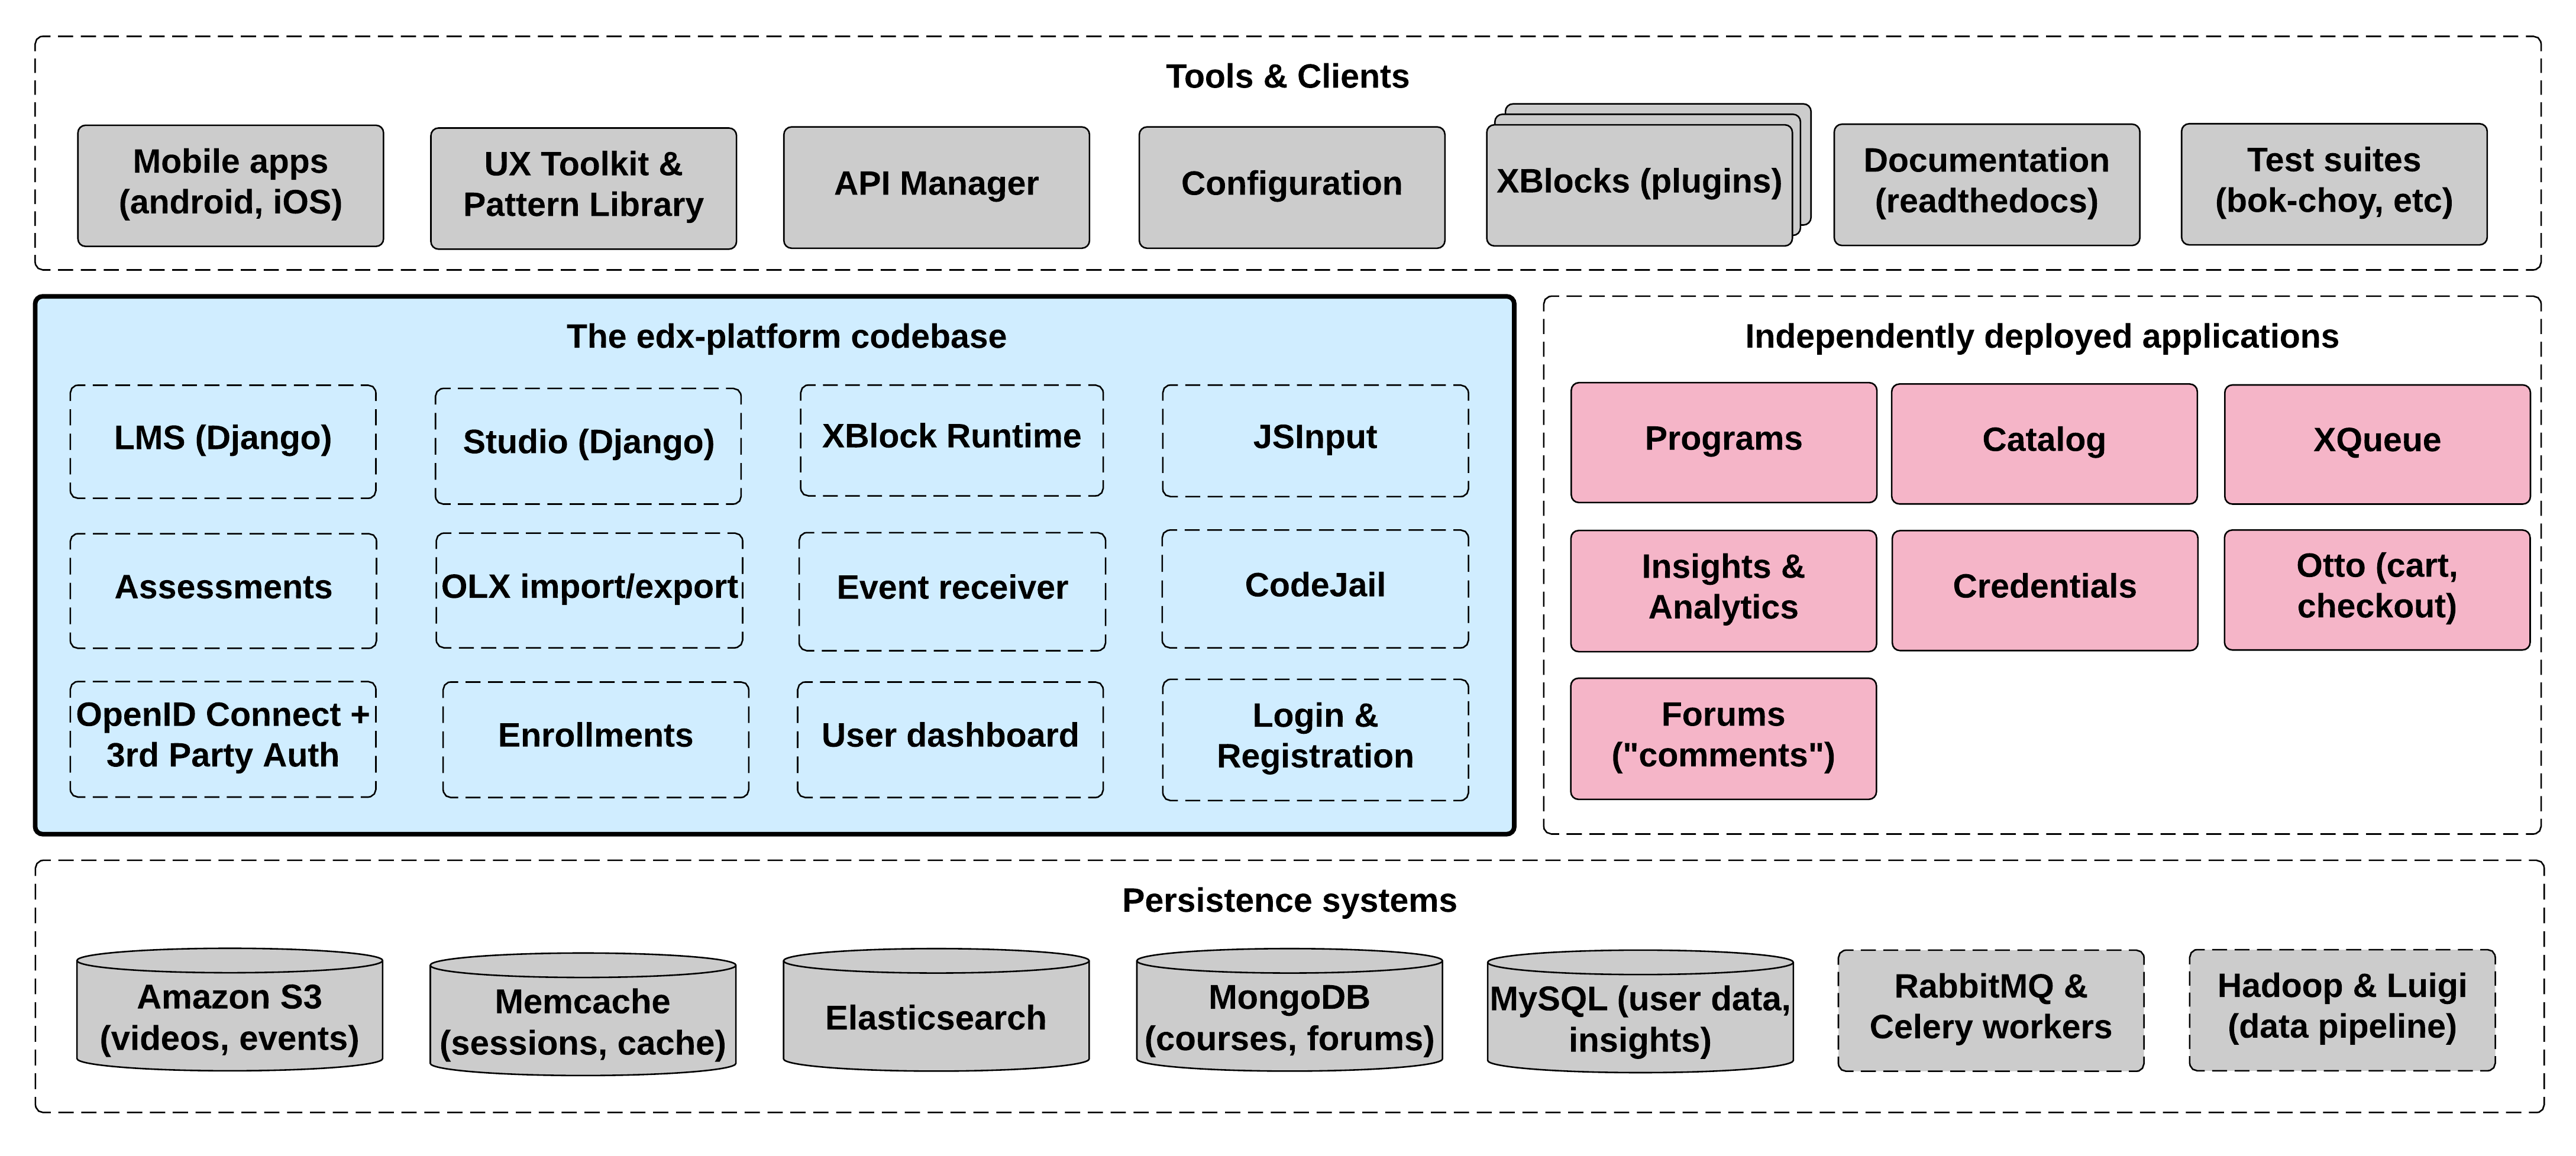
\includegraphics[width=0.8\textwidth, height=8cm]{edx-architecture}
\caption{Αρχιτεκονική Πλατφόρμας \textlatin{Open edX}}
\label{fig:edx_arch}
\end{figure}

\section{Κύρια Μέρη}
\subsection{Σύστημα Διαχείρισης Μάθησης (\textlatin{LMS})}\label{lms}
Το \textlatin{LMS} είναι η διεπαφή του λογισμικού \textlatin{Open edX}. Οι μαθητές παρακολουθούν μαθήματα χρησιμοποιώντας το \textlatin{LMS}. Το \textlatin{LMS} παρέχει επίσης ένα πίνακα ελέγχου-ρυθμίσεων για τους διδάσκοντες στο οποίο οι χρήστες που έχουν το ρόλο διαχειριστή ή προσωπικού μπορούν να έχουν πρόσβαση επιλέγοντας το ρόλο του eκπαιδευτή.

Το \textlatin{LMS} χρησιμοποιεί έναν αριθμό αποθηκευτικών χώρων για το περιεχόμενο που διανέμει. Το περιεχόμενο των μαθημάτων αποθηκεύεται σε μια βάση \textlatin{MongoDB}, ενώ τα βίντεο είναι δυνατό να προβάλλονται από το \textlatin{YouTube} ή το \textlatin{Amazon S3}. Τα δεδομένα ανά εκπαιδευόμενο αποθηκεύονται σε μια βάση \textlatin{MySQL}. Καθώς οι μαθητές μετακινούνται από μάθημα σε μάθημα και αλληλεπιδρούν με κάθε ένα από αυτά, τα δεδομένα που αφορούν σε αυτές τις αλληλεπιδράσεις συλλέγονται για περαιτέρω ανάλυση και εξαγωγή συμπερασμάτων.

Το \textlatin{LMS} αναλύεται περεταίρω στα παρακάτω επιμέρους τμήματα:
 \paragraph{Διεπαφή Χρήστη.} Ο κώδικας \textlatin{Django} από την πλευρά του εξυπηρετή χρησιμοποιεί το λογισμικό \textlatin{Mako} για τη παραγωγή διεπαφών και προτύπων (\textlatin{templates}). Ο κώδικας από την πλευρά του χρήστη είναι γραμμένος κυρίως σε \textlatin{JavaScript}, ενώ κάποια άλλα είναι γραμμένα σε \textlatin{Backbone.js framework}. Τα μέρη που χρησιμοποιούν \textlatin{CSS} υλοποιούνται με τη χρήση \textlatin{Bourbon - Sass frameworks}~\cite{edx_arch}.
 \paragraph{Περιήγηση Mαθημάτων.} Το λογισμικό \textlatin{Open edX} παρέχει μια απλή πρώτη σελίδα για την περιήγηση εντός των παρεχόμενων μαθημάτων. Ο ιστότοπος \textlatin{\url{https://edx.org}} από την άλλη, έχει ξεχωριστή αρχική σελίδα και διαφορετική για την περιήγηση εντός των μαθημάτων, οι οποίες όμως δεν είναι ανοικτού κώδικα.
 \paragraph{Δομή μαθημάτων.} Τα μαθήματα στο \textlatin{Open edX} αποτελούνται από μονάδες που ονομάζονται \textlatin{XBlocks}. Οι εκπαιδευτές μπορούν να γράψουν νέα \textlatin{XBlocks}, και με αυτό τον τρόπο να επεκτείνουν το σύνολο των βοηθημάτων για τα μαθήματά τους. Εκτός από τα \textlatin{XBlocks}, υπάρχουν και άλλοι τρόποι για να επεκταθεί η συμπεριφορά μαθημάτων:
\begin{itemize}
  \item Με τη χρήση εργαλείων \textlatin{LTI (Learning Tools Interoperability)}~\cite{lti}, για την ενσωματωση διαφόρων εργαλείων εκμάθησης σε ένα μάθημα \textlatin{Open edX}.
  \item Με την ενσωμάτωση κώδικα \textlatin{Python}, για την παρουσίαση εκπαιδευτικών εργασιών - προβλημάτων και την αξιολόγηση των απαντήσεων των εκπαιδευομένων. Ο κώδικας σε αυτή την περίπτωση, εκτελείται σε ασφαλές περιβάλλον (\textlatin{CodeJail})~\cite{edx_arch}.
  \item Τμήματα κώδικα \textlatin{JavaScript} μπορούν να ενσωματωθούν με τη χρήση του \textlatin{JS Input}.
  \item Ολόκληρα μαθήματα μπορούν να εισαχθούν και να εξαχθούν με τη χρήση του \textlatin{OLX (open learning XML)}, ενός ειδικού φορμάτ για την περιγραφή μαθημάτων στο \textlatin{open-edX}.
\end{itemize}

\subsection{\textlatin{Studio}}
Το \textlatin{Studio} είναι το περιβάλλον συγγραφής μαθημάτων. Οι εκπαιδευτές το χρησιμοποιούν για να δημιουργήσουν και να ενημερώσουν μαθήματα. Το \textlatin{Studio} γράφει τα μαθήματά του στην ίδια βάση δεδομένων \textlatin{Mongo} που χρησιμοποιεί το \textlatin{LMS}.

\subsection{Συζητήσεις}
H λειτουργια των συζητήσεων για τα μαθήματα ελέγχεται από ένα \textlatin{IDA}, που ονομάζεται \textlatin{comments} (ή \textlatin{forums}). Οι συζητήσεις είναι ένα από τα λίγα λειτουργικά μέρη του \textlatin{Open edX}, το οποίο δεν είναι γραμμένο σε γλώσσα \textlatin{Python}, αλλά σε \textlatin{Ruby} με τη χρήση του \textlatin{Sinatra framework}. Το \textlatin{LMS} χρησιμοποιεί ένα \textlatin{API}, το οποίο χρησιμοποιεί το \textlatin{comments service} για να ενσωματώσει τις συζητήσεις στην εμπειρία των μαθημάτων. Η υπηρεσία αυτή περιλαμβάνει μια διαδικασία κοινοποίησης, που στέλνει ειδοποιήσεις στους εγγεγραμμένους μαθητές, σχετικά με ενημερώσεις σε θέματα ενδιαφέροντος.

\subsection{Ενσωμάτωση Λειτουργικότητας Φορητών Συσκευών} Το \textlatin{Open edX} περιλαμβάνει μια εφαρμογή για κινητά, διαθέσιμη για \textlatin{iOS} και \textlatin{Android}, η οποία επιτρέπει στους μαθητές να παρακολουθούν βίντεο-μαθήματα και πολλά άλλα. Το \textlatin{EdX} αναπτύσσει ενεργά την εφαρμογή για κινητά.

\subsection{\textlatin{Analytics}}
Γεγονότα τα οποία περιγράφουν την αλληλεπίδραση των μαθητών, συλλέγονται από το \textlatin{analytics framework} του \textlatin{Open edX}. Τα συμβάντα αποθηκεύονται ως \textlatin{JSON} σε \textlatin{S3}, υποβάλλονται σε επεξεργασία χρησιμοποιώντας εργαλεία \textlatin{Hadoop} και στη συνέχεια τα συγκεντρωτικά αποτελέσματα αποθηκεύονται στην \textlatin{MySQL}. Τα αποτελέσματα διατίθενται μέσω ενός \textlatin{REST API} στo \textlatin{Insights}, ένα \textlatin{IDA} που χρησιμοποιείται από τους εκπαιδευτές και τους διαχειριστές για τη διερεύνηση δεδομένων, τα οποία τους επιτρέπουν να γνωρίζουν τι κάνουν οι μαθητές τους και πώς χρησιμοποιούνται τα μαθήματά τους. Ένα διάγραμμα των στοιχείων και των τεχνολογιών που αποτελούν την αρχιτεκτονική του \textlatin{Open edX analytics} φαίνεται στο παρακάτω σχήμα~\ref{fig:edx_analytics_arch}:
\begin{figure}[!htbp]
\centering
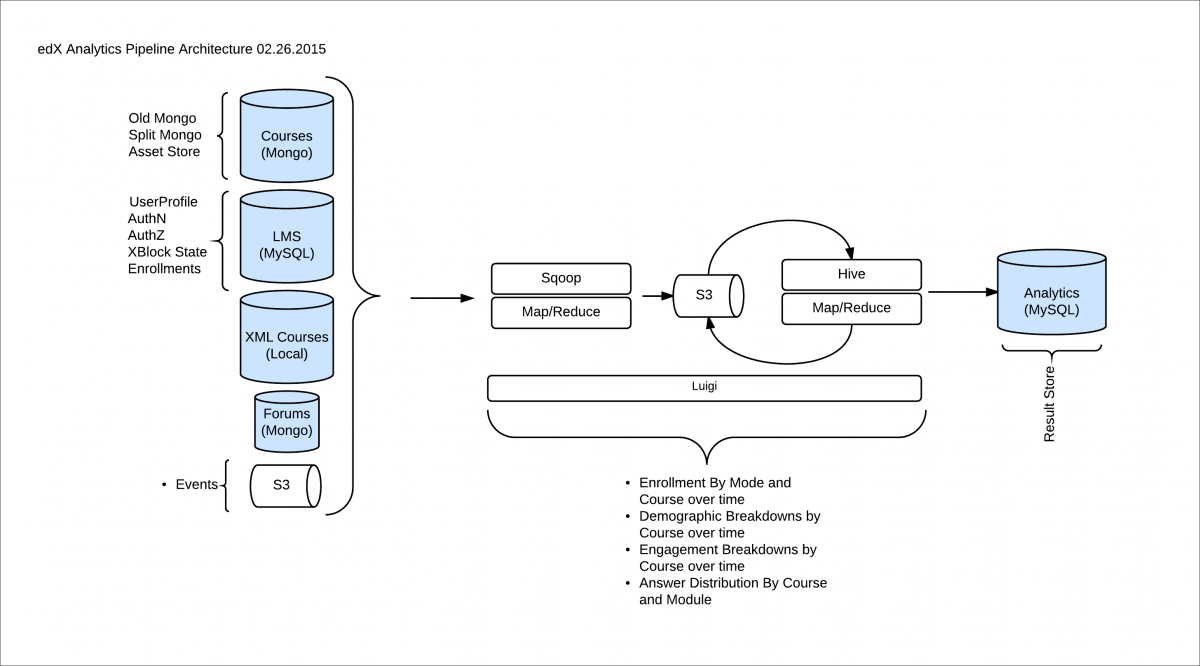
\includegraphics[width=0.8\textwidth, height=8cm]{edx-architecture-analytics}
\caption{Αρχιτεκονική \textlatin{Open edX analytics}}
\label{fig:edx_analytics_arch}
\end{figure}

\subsection{Λειτουργίες Παρασκηνίου}
Ορισμένες εργασίες είναι αρκετά μεγάλες ώστε να εκτελούνται από από τις ίδιες τις εφαρμογές ιστού. Για αυτό το λόγο, τέτοιου είδους εργασίες ανατίθενται σε ξεχωριστές διεργασίες στο παρασκήνιο. Αυτές οι εργασίες τοποθετούνται σε ουρά και διανέμονται με τη βοήθεια των \textlatin{Celery} και \textlatin{RabbitMQ frameworks}. Παραδείγματα τέτοιων εργασιών περιλαμβάνουν:
\begin{itemize}
  \item Βαθμολόγηση μαθημάτων
  \item Αποστολή μαζικών μηνυμάτων ηλεκτρονικού ταχυδρομείου (με το \textlatin{Amazon SES})
  \item Δημιουργία αναφορών διανομής απαντήσεων
  \item Αποστολή πιστοποιητικών ολοκλήρωσης μαθημάτων
\end{itemize}

\subsection{Αναζήτηση}
Το \textlatin{Open edX} χρησιμοποιεί το \textlatin{Elasticsearch} για αναζήτηση σε πολλαπλά επίπεδα, συμπεριλαμβανομένης της αναζήτησης εντός των μαθημάτων και των συζητήσεων.

\subsection{Επιπλέον Λειτουργικότητα}
Εκτός από τα όσα αναθέρθηκαν παραπάνω, το \textlatin{Open edX} διαθέτει επίσης επιπλέον δυνατότητες, όπως τη διαχειρίση λειτουργιών ηλεκτρονικού εμπορίου~\cite{edx_arch}.

Το παρόν πραγματεύεται την ανάπτυξη ενός ενδεικτικού ιστοτόπου μαθήματος στην πλατφόρμα \textlatin{Open edX}. Στα επόμενα παρουσιάζεται η διαδικασία εγκατάστασης της πλατφόρμας με τη χρήση αυτοματοποιημένων εργαλείων ανάπτυξης, ενώ γίνεται και μια συνοπτική αναφορά στα εργαλεία που χρησιμοποιήθηκαν κατά την εγκατάσταση αυτή.

\chapter{Εγκατάσταση της Πλατφόρμας \textlatin{Open edX}}\label{ch3}
Για την εγκατάσταση της εν λόγω πλατφόρμας χρησιμοποιήθηκε αριθμός εργαλείων, τα οποία στην πλειονότητά τους βρίσκονται διαθέσιμα δωρεάν στο Διαδίκτυο (\textlatin{Open Source Software}). Στα επόμενα γίνεται μια σύντομη αναφορά στα εργαλεία που χρησιμοποιήθηκαν και στη διαδικασία της εγκατάστασης.

\section{\textlatin{\textlatin{Vagrant (Open Source VM Provissioner)}}}\label{vagrant}
Το \textlatin{Vagrant} είναι ένα εργαλείο δημιουργίας και διαχείρησης εικονικών μηχανών με τη χρήση μιας εξαιρετικά απλοποιημένης διαδικασίας~\cite{vagrant_by_hashicorp}. Το εργαλείο αυτό δίνει έμφαση στην αυτοματοποιημένη διαχείριση των εικονικών μηχανών και μειώνει σημαντικά το χρόνο δημιουργίας και παραμετροποίησης ενός \textlatin{development server}.

Είναι γραμμένο στη γλώσσα προγραμματισμού \textlatin{Ruby} και αποτελεί έναν ενιαίο τρόπο επικοινωνίας με δίάφορους \textlatin{providers} εικονικών μηχανών (όπως \textlatin{VirtualBox, VMware, AWS} κ.α.). Με τον τρόπο αυτό είναι δυνατή η δημιουργία εικονικών μηχανών με τις επιθυμητές παραμέτρους στον μικρότερο δυνατό χρόνο. Παράλληλα, για την εγκατάσταση πακέτων λογισμικού αλλά και παραμετροποίηση σε επίπεδο λειτουργικού συστήματος (ΛΣ), είναι δυνατή η συνεργασία με ευρέως διαδεδομένα \textlatin{provisioning tools}, όπως \textlatin{Chef, Puppet, Ansible} ακόμα και με απλά \textlatin{shell scripts}.

Το μεγαλύτερο ίσως πλεονέκτημα του υπόψη εργαλείου είναι η δυνατότητα παροχής στους προγραμματιστές ενός ενιαίου περιβάλλοντος, το οποίο είναι σταθερό και όσο κοντά γίνεται στο παραγωγικό εξυπηρετητή. Επίσης επειδή η παραμετροποίηση γίνεται με αυτόματο τρόπο, αφαιρείται από τους προγραμματιστές το βάρος της δημιουργίας, συντήρησης και αποσφαλμάτωσης του περιβάλλοντος ανάπτυξης.

Η αρχή λειτουργίας του \textlatin{Vagrant} στηρίζεται στην ύπαρξη μιας εικονικής μηχανής στελέχους (\textlatin{template/vagrant box}), η οποία είναι διαθέσιμη από τα επίσημα αποθετήρια \textlatin{\url{https://vagrantcloud.com/boxes/search}} είτε μπορεί να είναι δική μας. Κατόπιν μέσω μιας διαδικασίας κλωνοποίησης και εφαρμογής παραμέτρων, εντελώς διαφανούς για το χρήστη, αποδίδεται η εικονική μηχανή.

Όλα τα παραπάνω γίνονται με την εκτέλεση της εντολής \textlatin{\texttt{vagrant}} ακολουθούμενης από το αντίστοιχο \textlatin{switch}. Για παράδειγμα, η παρακάτω ακολουθία εντολών κατεβάζει μια εικονική μηχανή \textlatin{ubuntu 64bit} από το επίσημο αποθετήριο και την θέτει σε λειτουργία με τη βοήθεια του \textlatin{VirtualBox}.
\selectlanguage{english}
\begin{lstlisting}
  $ vagrant box add ubuntu/xenial64
  $ vagrant init
  $ vagrant up --provider=virtualbox
\end{lstlisting}
\selectlanguage{greek}
Για τη φιλοξενία του ιστοτόπου της εργασίας χρησιμοποιήθηκε μια μηχανή \textlatin{ubuntu 16.04 64bit} από το επίσημο αποθετήριο. Χρησιμοποιήθηκε ως \textlatin{Virtualization provider} το λογισμικό \textlatin{VirtualBox}. Στην συνέχεια με τη χρήση \textlatin{shell provissioner} έγινε η εγκατάσταση και παραμετροποίηση των απαραίτητων πακέτων και ρυθμίσεων του λειτουργικού συστήματος. Με τη χρήση του ίδιου \textlatin{provissioner}, μέσω της κλήσης του \textlatin{bash script} του Παραρτήματος~\ref{AppB} πραγματοποιήθηκαν τα τελικά στάδια εγκατάστασης και παραμετροποίησης της πλατφόρμας.

Όλα τα παραπάνω ορίζονται στο αρχείο \textlatin{\texttt{Vagrantfile}} το οποίο παρατίθεται στο Παράρτημα~\ref{AppA}.

\section{Εργαλείο Αυτοματοποίησης \textlatin{Ansible}}\label{ansible}
Το \textlatin{ansible} είναι ένα λογισμικό ανοιχτού κώδικα, το οποίο χρησιμοποιείται για την αυτοματοποίηση των διεργασιων εγκατάστασης λογισμικού, διαχείρησης παραμέτρων και διάθεσης υπηρεσιών~\cite{wikipedia_2019}.

Το όνομα \textlatin{"Ansible"} αναφέρεται σε ένα φανταστικό σύστημα άμεσης υπερ-διαστημικής επικοινωνίας (όπως αναφέρεται στο \textlatin{Ender's Game} (1985) του \textlatin{Orson Scott Card}~\cite{wikipedia_2019}), το οποίο είχε εμπνευστεί από τη νουβέλα της \textlatin{Ursula K. Le Guin, Rocannon's World (1966)}~\cite{worldcat}.

Όπως με τα περισσότερα λογισμικά αυτού του τύπου, το \textlatin{Ansible} έχει δύο τύπους εξυπηρετητών, με τους οποίους ανταλλάσει δεδομένα: τους ελεγκτές και τους ελεγχόμενους κόμβους. Το λογισμικό \textlatin{Ansible}, το οποίο τρέχει στην μηχανή ελεγκτή, συνδέεται στους προς διαχείρηση κόμβους, με τη χρήση \textlatin{SSH, remote PowerShell} είτε άλλων \textlatin{remote APIs}. Η \textlatin{Ansible} αναγνωρίζει τους προς διαχείρηση κόμβούς με τη χρήση ειδικών αρχείων (\textlatin{Inventory}).

Σε αντίθεση με διάφορα λογισμικά του είδους, όπως τα \textlatin{Chef, Puppet, CFEngine} το \textlatin{Ansible} δε χρειάζεται την εγκατάσταση συγκεκριμένου \textlatin{agent} στα μηχανήματα στόχους (\textlatin{agentless architecture}~\cite{wikipedia_2019}). Σε ένα τέτοιο είδος αρχιτεκτονικής, οι εξυπηρετητές δεν επιβαρύνονται με επιπλέον υπηρεσίες ή λογισμικό, τα οποία τρέχουν στο παρασκήνιο και απορροφούν πόρους.

\section{Διαδικασία Εγκατάστασης}
Μετά την εγκατάσταση της εικονικής μηχανής με τη χρήση του \textlatin{Vagrantfile}, όπως περιγράφηκε στο~\ref{vagrant}, ακολουθήθηκε η διαδικασία εγκατάστασης της πλατφόρμας με την κλήση του \textlatin{bash script} του Παραρτήματος~\ref{AppB}. Επιλέχθηκε η \textlatin{native installation}, έναντι των \textlatin{fullstack} ή \textlatin{devstack}, καθώς είναι η πιο πλήρης και μπορεί να εγκατασταθεί σε παραγωγικό εξυπηρετητή χωρίς ιδιαίτερες μετατροπές. Για την έκδοση του \textlatin{Open edX} επιλέχθηκε η προηγούμενη σταθερή έκδοση (\textlatin{Ginkgo2} αντί \textlatin{Hawthorn}), καθώς είναι πιο δοκιμασμένη και απαιτεί λιγότερο χρόνο σε αποσφαλμάτωση.

Οι 10 πρώτες γραμμές του \textlatin{bash script} διενεργούν αρχικούς ελέγχους και δημιουργούν απαραίτητους φακέλους. Στη συνέχεια εγκαθιστούνται στους αντίστοιχους φακέλους απαραίτητα \textlatin{components} του \textlatin{Open edX}. Στις γραμμές 40-141 εισάγεται ένα πιστοποιητικό που αφορά σε πακέτα προς εγκατάσταση (αποτυγχάνει μέσω της αυτοματοποιημένης εγκατάστασης).

Στη συνέχεια ορίζεται η προς εγκατάσταση έκδοση του \textlatin{Open edX (Ginkgo2)} και μεταφορτώνεται το \textlatin{script} εγκατάστασης από το επίσημο αποθετήριο λογισμικού. Οι γραμμές 162-313 δημιουργούν ένα αρχείο \textlatin{patch}, το οποίο χρησιμοποιείται αργότερα για την τροποποίηση κάποιων αρχείων του λογισμικού, τα οποία δημιουργούν σφάλματα κατά την εγκατάσταση. Τέλος στις γραμμές 315-326 γίνεται μεταφόρτωση του λογισμικού \textlatin{Open edX}, εφαρμόζεται το προαναφερθέν \textlatin{patch} και καλείται η \textlatin{ansible} για την ολοκλήρωση της αυτοματοποιημένης εγκατάστασης. Το αποτέλεσμα της εγκατάστασης είναι η αρχική σελίδα της πλατφόρμας του \textlatin{Open edX}~\ref{fig:edx_landing}:
\begin{figure}[!htbp]
\centering
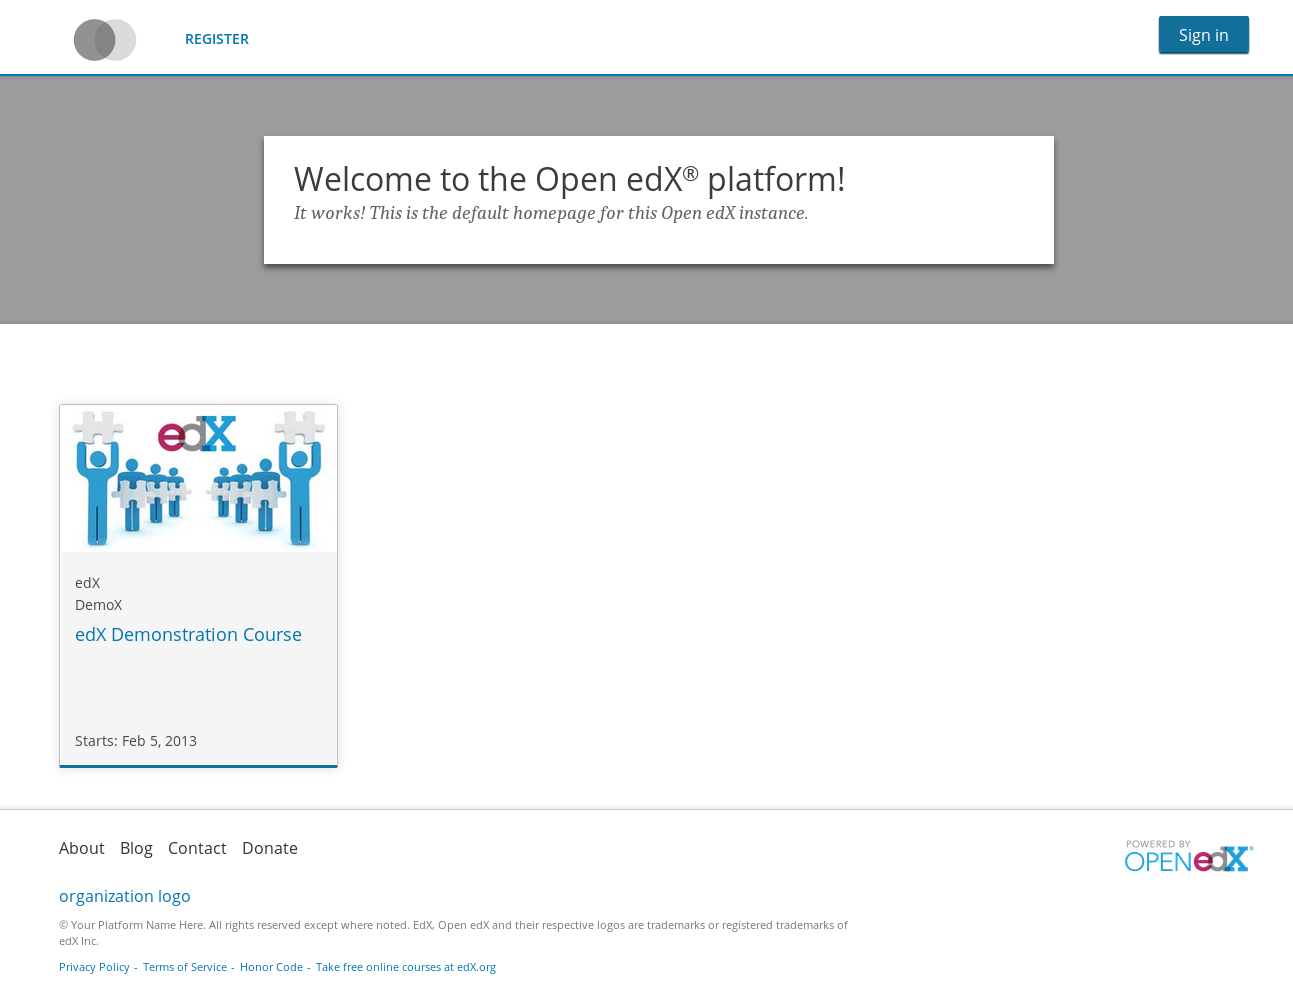
\includegraphics[width=0.8\textwidth, height=8cm]{openedx-start}
\caption{Αρχική Σελίδα \textlatin{Open edX}}
\label{fig:edx_landing}
\end{figure}

\section{Συνοπτική Περιγραφή Λειτουργιών Πλατφόρμας}
\subsection{Εισαγωγή}\label{edx_intro}
Με το πέρας της εγκατάστασης είναι δυνατή η πρόσβαση των λειτουργιών της πλατφόρμας, όπως παρακάτω~\cite{confluence_1}:
\begin{itemize}
  \item \textlatin{LMS: \url{http://192.168.33.10/}}
  \item \textlatin{Studio: \url{http://192.168.33.10:18010/}}
  \item \textlatin{Django Admin: \url{http://192.168.33.10/admin}}
\end{itemize}

Οι υπάρχοντες λογαριασμοί, οι οποίοι ενεργοποιούνται με την εγκατάσταση είναι οι παρακάτω~\cite{confluence_2}:
\begin{itemize}
  \item \textlatin{\texttt{staff@example.com}} Ένας χρήστης του \textlatin{LMS/Studio} με δικαιώματα δημιουργίας και αλλαγών μαθημάτων.
  \item \textlatin{\texttt{verified@example.com}} Ένας δοκιμαστικός χρήστης του \textlatin{LMS}, με το ρόλο του εκπαιδευομένου (\textlatin{certificate verification}).
  \item \textlatin{\texttt{audit@example.com}} Ένας δοκιμαστικός χρήστης του \textlatin{LMS}, με το ρόλο του εκπαιδευομένου (\textlatin{course auditing}).
  \item \textlatin{\texttt{honor@example.com}} Ένας δοκιμαστικός χρήστης του \textlatin{LMS}, με το ρόλο του εκπαιδευομένου (\textlatin{honor certificate verification}).
\end{itemize}

Όλοι οι παραπάνω χρήστες έχουν κωδικό εισόδου \textlatin{\texttt{"edx"}}.

\subsection{\textlatin{Django Admin Panel}}\label{edx_panel}
Το \textlatin{Django Admin Panel} χρησιμοποιείται για τη διαχείρηση της πλατφόρμας. Γενικότερα απαιτεί εξοικείωση με την πλατφόρμα και τον τρόπο λειτουργίας της. Από εδώ μπορεί να γίνει διαχείρηση χρηστών, εφαρμογή θεμάτων, δημιουργία \textlatin{subdomain}, εφαρμογή κανόνων για ένα σύνολο μαθημάτων κ.α. Γενικά αποτελεί το δυνατότερο εργαλείο παραμετροποίησης όλης της πλατφόρμας. Οι χρήστες που περιγράφτηκαν στο τμήμα~\ref{edx_intro} δεν μπορούν να χρησιμοποιηθούν για το \textlatin{Django Admin}. Για την ενεργοποίηση δικαιωμάτων \textlatin{admin} ενός υπαρχοντος χρήστη (π.χ. \textlatin{staff}), ακολουθείται η παρακάτω διαδικασία από το \textlatin{bash shell}:
\selectlanguage{english}
\begin{lstlisting}
  $ sudo -H -u edxapp bash
  $ source /edx/app/edxapp/edxapp_env
  $ source /edx/app/edxapp/venvs/edxapp/bin/activate
  $ cd /edx/app/edxapp/edx-platform
  $ ./manage.py lms manage_user staff staff@example.com --staff --superuser --settings=devstack
\end{lstlisting}
\selectlanguage{greek}

Η αρχική σελίδα του \textlatin{admin panel} φαίνεται στην εικόνα~\ref{fig:django-login}. Μετά την επιτυχή είσοδο στη σελίδα του \textlatin{admin panel} ο διαχειριστής μπαίνει στη σελίδα διαχείρησης του ιστοτόπου~\ref{fig:django-landing}.
\begin{figure}[!htbp]
\centering
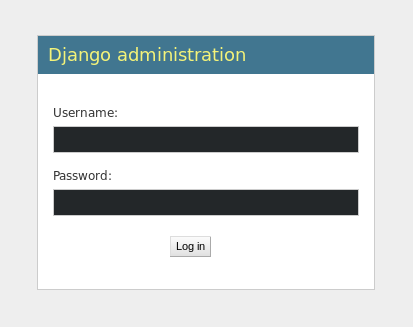
\includegraphics[width=0.9\textwidth, height=8cm]{django-login}
\caption{Φόρμα Εισόδου \textlatin{admin panel}}
\label{fig:django-login}
\end{figure}

\begin{figure}[!htbp]
\centering
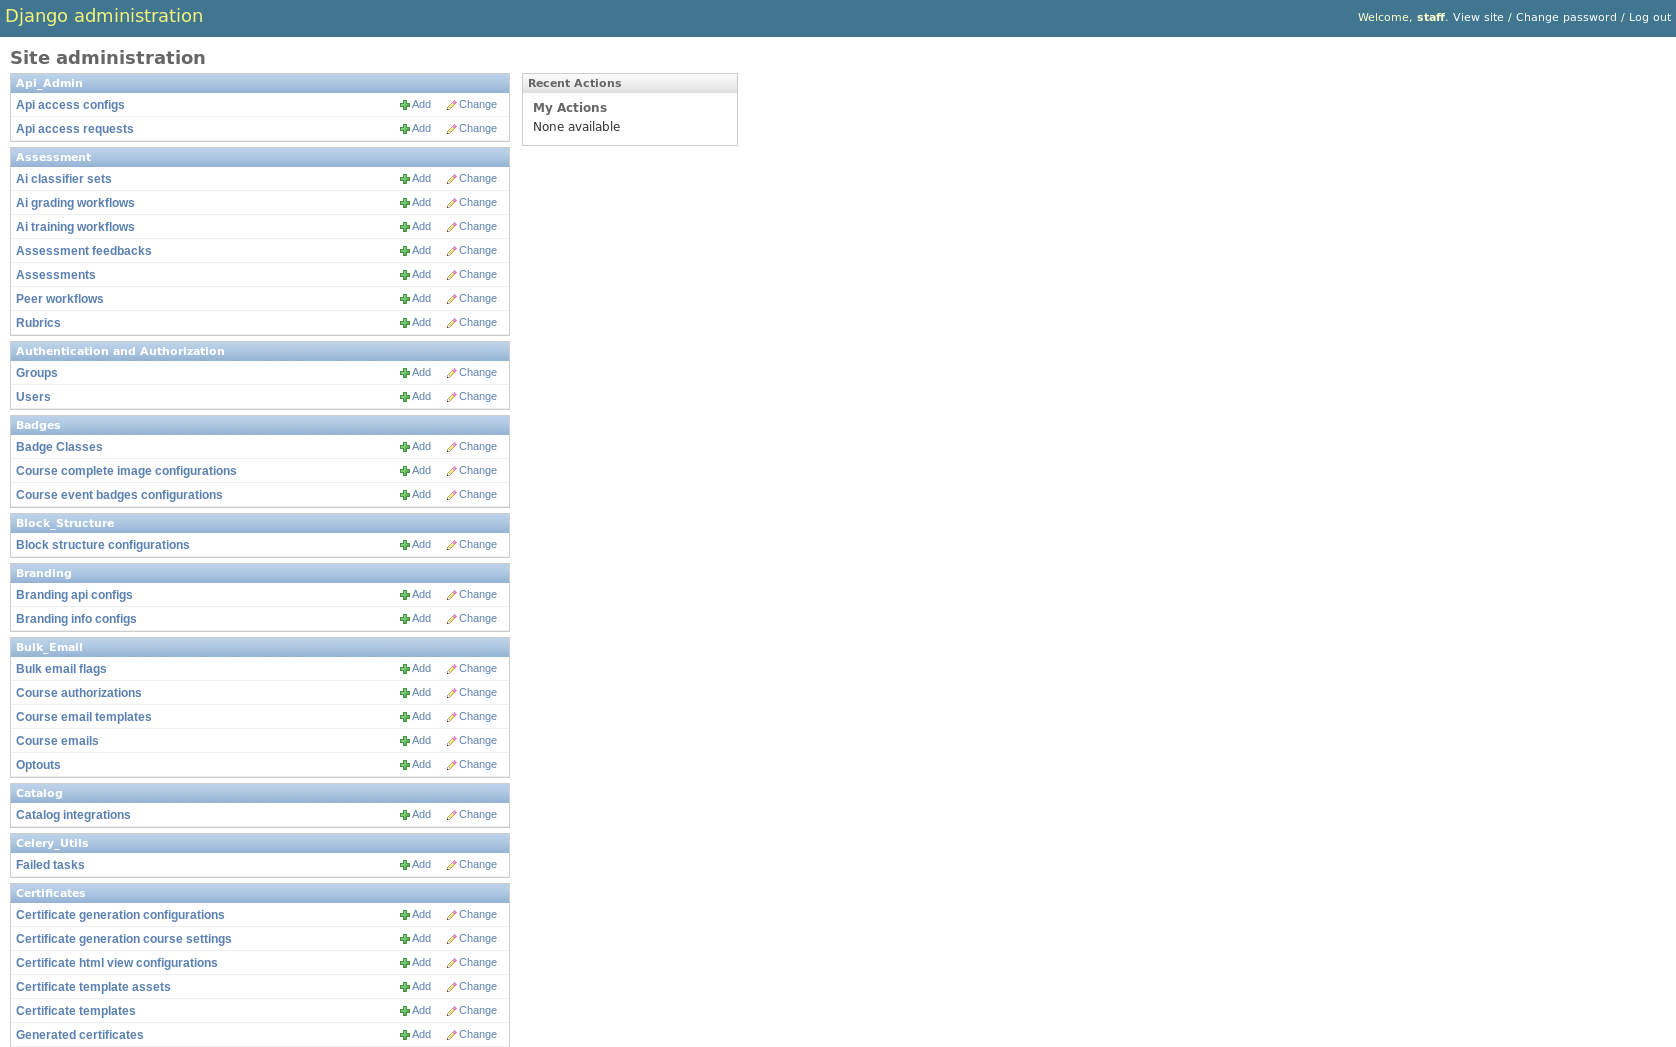
\includegraphics[width=0.9\textwidth, height=10cm]{django-landing-page}
\caption{\textlatin{Admin panel}}
\label{fig:django-landing}
\end{figure}

Οι λειτουργικότητες, που αφορούν στο \textlatin{LMS} και \textlatin{Studio}, αναλύονται στα αντίστοιχα τμήματα~\ref{lms_use} και~\ref{studio}.

\chapter{Δημιουργία Ενδεικτικού Ιστοτόπου Μαθήματος}\label{ch4}
\section{Εισαγωγή}
Στη συνέχεια γίνεται σύντομη αναφορά στη διαδικασία δημιουργίας ενός ιστοτόπου μαθήματος (\textlatin{microsite}) της πλατφόρμας \textlatin{Open edX}. Έπειτα παρουσιάζεται συνοπτικά η λειτουργικότητα του ιστοτόπου αυτού. Παρατίθενται για αυτό το σκοπό ανάλογα \textlatin{screenshots} με επεξηγήσεις για τις κύριες λειτουργίες.

Τα \textlatin{microsites} είναι \textlatin{subdomains} του κύριου \textlatin{domain} της πλατφόρμας \textlatin{Open edX}. Αυτά τα \textlatin{subdomains} βοηθούν στην καλύτερη ομαδοποίηση του \textlatin{MOOC} περιεχομένου, με τέτοιο τρόπο ώστε να είναι εφικτός ο διαχωρισμός των μαθημάτων με βάση συγκεκριμένα κριτήρια~\cite{microsites_2}. Τέτοιοι διαχωρισμοί μπορεί να είναι:
\begin{itemize}
  \item Μαθήματα ενός συγκεκριμένου εκπαιδευτή, από τα υπόλοιπα διαθέσιμα στην πλατφόρμα.
  \item Μαθήματα μιας συγκεκριμένης σχολής, ξεχωριστά από των υπολοίπων
  \item Μαθήματα ενός τμήματος μόνο.
  \item Μαθήματα μιας εταιρίας, ξεχωριστά από μάθήματα με παρόμοια αντικέιμενα.
  \item Αρχική σελίδα ενός και μόνου μαθήματος, το οποίο προβάλει καλύτερα το μάθημα και έλκει την προσοχή των μαθητών.
\end{itemize}
Με αυτό τον τρόπο οι μαθητές μπορούν να βρουν εύκολα ανάμεσα στα διαθεσιμα μαθήματα, αυτά που τους ενδιαφέρουν, χωρίς να είναι αναγκασμένοι να διατρέξουν όλη τη λίστα των μαθημάτων.

\subsection{Πλεονεκτήματα των \textlatin{microsites}}
Εκτός από την ομαδοποίηση των μαθημάτων με συγκεκριμένα κριτήρια, όπως περιγράφηκε παραπάνω, η χρήση των \textlatin{microsites} παρέχει επιπρόσθετα πλεονεκτήματα. Για παράδειγμα κάθε \textlatin{microsite} μπορεί να έχει το δικό του θέμα, ταπετσαρία ή γραμματοσειρά. Επιπρόσθετα κάθε \textlatin{microsite} μπορεί να έχει διαφορετικά σύνολα από λειτουργικά \textlatin{XBlocks}, για παράδειγμα διαφορετικά για μαθήματα Χημείας ή Μαθηματικών. Τέλος είναι δυνατή η ενεργοποίηση διαφορετικών μεθόδων αποπληρωμής, για τις παρεχόμενες υπηρεσίες της πλατφόρμας σε κάθε \textlatin{microsite}.

\section{Δημιουργία του Ιστοτόπου Μαθήματος}
Για τη δημιουργία του ιστοτόπου μαθήματος ακολουθήθηκε η επίσημη τεκμηρίωση της πλατφόρμας~\cite{edxdata_package_1} και ~\cite{microsites_1}. Αρχικά τροποποιήθηκε το \textlatin{microsite template}, το οποίο υπάρχει στον κώδικα του \textlatin{Open edX} στη διαδρομή \textlatin{\texttt{/edx/app/edxapp/edx-platform/ common/test/test\_sites/test\_site}}, έτσι ώστε να αντιστοιχεί στο επιθυμητό αποτέλεσμα. Οδηγός για τις απαραίτητες αλλαγές στάθηκε το~\cite{microsites_1}. Χρησιμοποιήθηκαν επίσης, τα \textlatin{logo} του εργαστηρίου από την επίσημη ιστοσελίδα (\textlatin{\url{https://www.netmode.ntua.gr}}).

Για την ενεργοποίηση του \textlatin{microsite} έγιναν οι απαραίτητες αλλαγές στο αρχείο \textlatin{\texttt{/edx/ app/edxapp/edx-platform/lms.env.json}}~\cite{microsites_1} με την προσθήκη των γραμμών που το ορίζουν σε μορφή \textlatin{json}:
\selectlanguage{english}
\inputminted[linenos, fontsize=\scriptsize, breaklines, baselinestretch=1, firstline=24, lastline=55]{json}{edx-microsite/README.md}
\selectlanguage{greek}

Η παραπάνω διαδικασία είναι δυνατό να πραγματοποιηθεί και από το \textlatin{Django Admin Panel}~\ref{edx_panel}, μέσω των αντίστοιχων επιλογών που διατίθενται για αυτό το σκοπό. Σε αυτή την περίπτωση επιλέγουμε \textlatin{\texttt{Add site}}~\ref{fig:django-new-site} και έπειτα κάνουμε επικόλληση το \textlatin{json} που περιγράφηκε παραπάνω~\ref{fig:django-site-conf}.

\begin{figure}[!htbp]
\centering
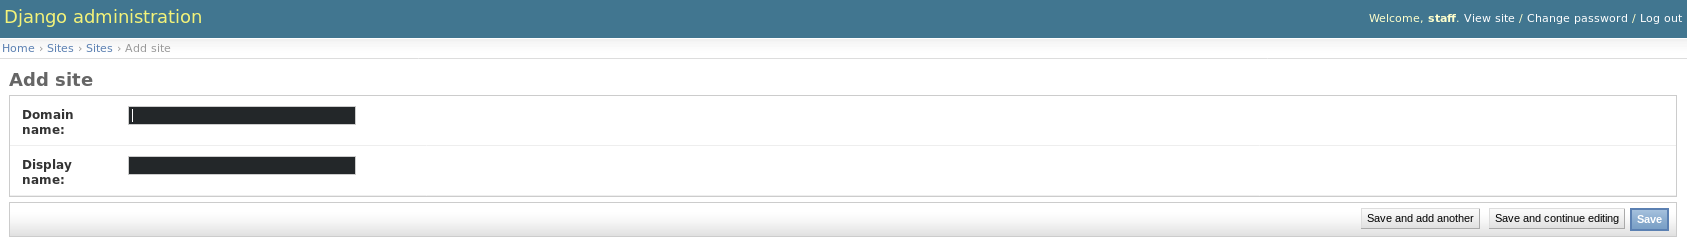
\includegraphics[width=0.8\textwidth, height=4cm]{django-new-site}
\caption{Σελίδα Δημιουργίας Ιστοτόπου}
\label{fig:django-new-site}
\end{figure}

\begin{figure}[!htbp]
\centering
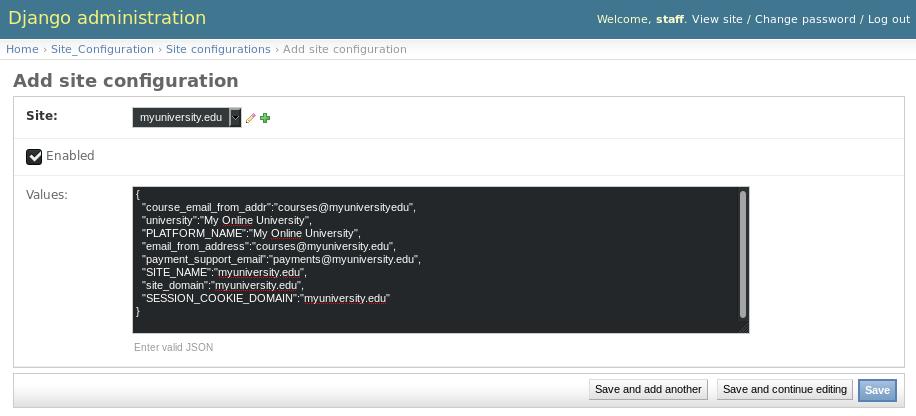
\includegraphics[width=0.8\textwidth, height=8.5cm]{django-site-conf}
\caption{Σελίδα Εισαγωγής Ρυθμίσεων Ιστοτόπου}
\label{fig:django-site-conf}
\end{figure}

Η ενεργοποίηση του ιστοτόπου πραγματοποίηθηκε στη συνέχεια με \textlatin{static assets recompile} και επανεκκίνηση των υπηρεσιών της πλατφόρμας~\cite{lawrence_mcdaniel_2018}:
\selectlanguage{english}
\begin{lstlisting}
  $ sudo -H -u edxapp bash
  $ source /edx/app/edxapp/edxapp_env
  $ source /edx/app/edxapp/venvs/edxapp/bin/activate
  $ cd /edx/app/edxapp/edx-platform
  $ paver update_assets
  $ sudo /edx/bin/supervisorctl restart all
\end{lstlisting}
\selectlanguage{greek}
Με αυτό τον τρόπο δημιουργήθηκε η αρχική σελίδα του \textlatin{microsite}~\ref{fig:microsite_landing}, σε αντιπαράθεση με την αρχική σελίδα της πλατφόρμας~\ref{fig:edx_landing}:
\begin{figure}[!htbp]
\centering
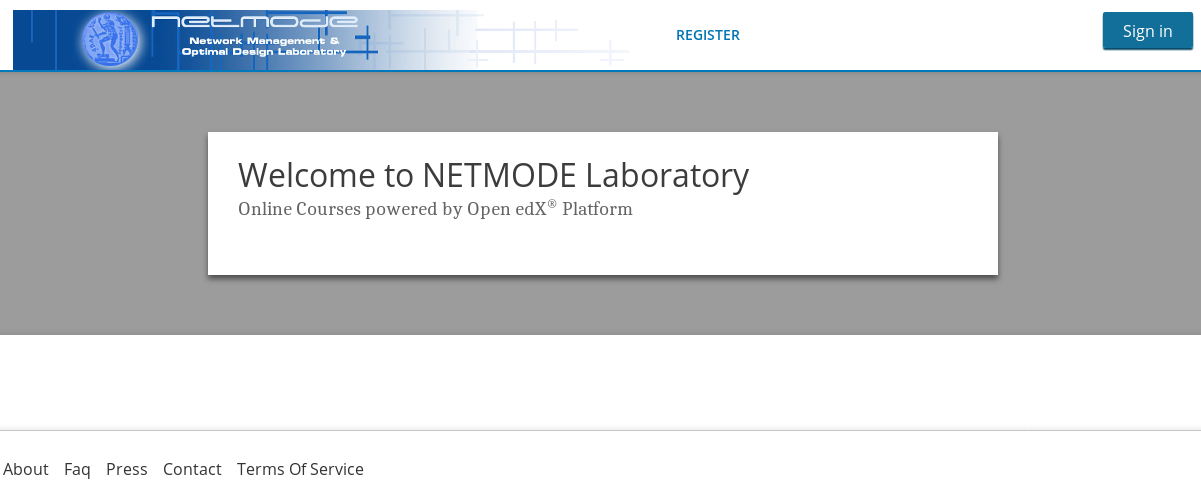
\includegraphics[width=0.8\textwidth, height=8.5cm]{microsite-landing}
\caption{Αρχική Σελίδα \textlatin{edX microsite}}
\label{fig:microsite_landing}
\end{figure}

\section{Δημιουργία Eνδεικτικού Μαθήματος}\label{studio}
Η αρχική σελίδα του \textlatin{microsite} εμφανίζεται κενή μαθημάτων εάν δεν ορίσουμε ή δημιουργήσουμε ένα. Για τη δημιουργία των μαθημάτων χρησιμοποιείται το εργαλείο \textlatin{studio}. Η αρχική σελίδα του εργαλείου, αφού αποκτήσουμε πρόσβαση όπως το τμήμα~\ref{edx_intro}, φαίνεται στην εικόνα~\ref{fig:edx-studio-landing}
\begin{figure}[!htbp]
\centering
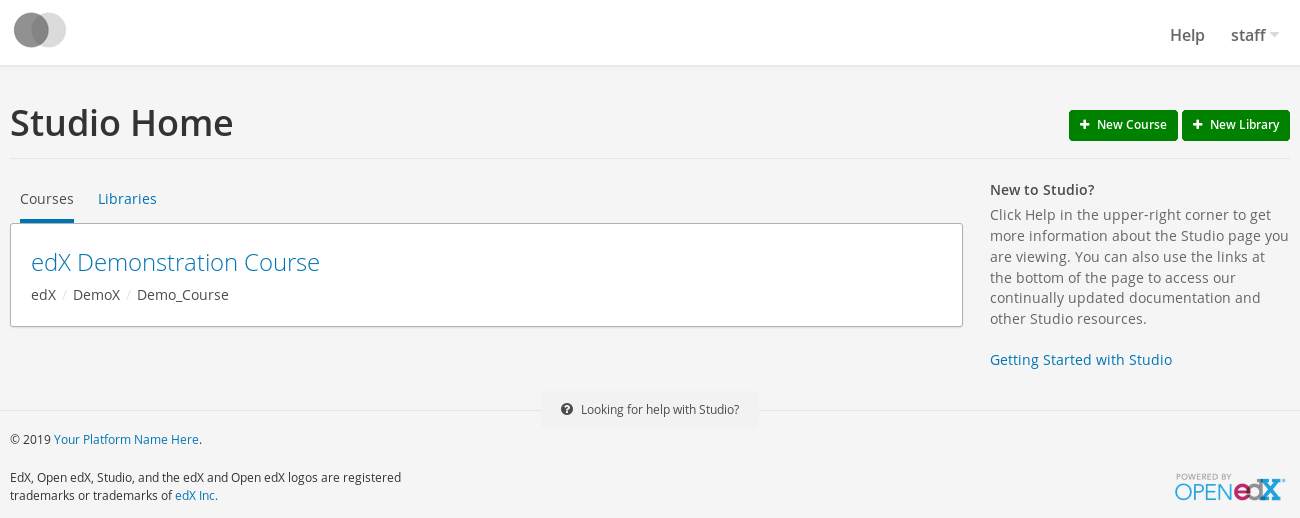
\includegraphics[width=0.8\textwidth, height=8.5cm]{edx-studio-landing}
\caption{Αρχική Σελίδα \textlatin{edX studio}}
\label{fig:edx-studio-landing}
\end{figure}

Από αυτή τη σελίδα είναι δυνατή η αλλαγή ενός υπαρχοντος μαθήματος (προσθήκη περιεχομένου ή αλλαγή ρυθμίσεων) είτε η προσθήκη ενός νέου~\cite{edxdata_package_2}. Η επιλογή γίνεται μέ τη χρήση των αντίστοιχων πλήκτρων πάνω στα δεξίά της οθόνης. Εφόσον επιλεγεί η δημιουργία ενός νέου μαθήματος, οδηγούμαστε στην επόμενη οθόνη, όπου μπορούμε να ορίσουμε τα βασικά στοιχεία του νέου μαθήματος (εικόνα~\ref{fig:edx-studio-new-course}). Η βασική παράμετρος ή οποία πρέπει να οριστεί σωστά, είναι το \textlatin{Organization}. Εάν θέλουμε το νέο μάθημα να εμφανίζεται στο \textlatin{microsite} που δημιουργήσαμε προηγουμένως πρέπει αυτή η παράμετρος να έχει ίδια τιμή με του \textlatin{course\_org\_filter} στις ρυθμίσεις του \textlatin{microsite}.
\begin{figure}[!htbp]
\centering
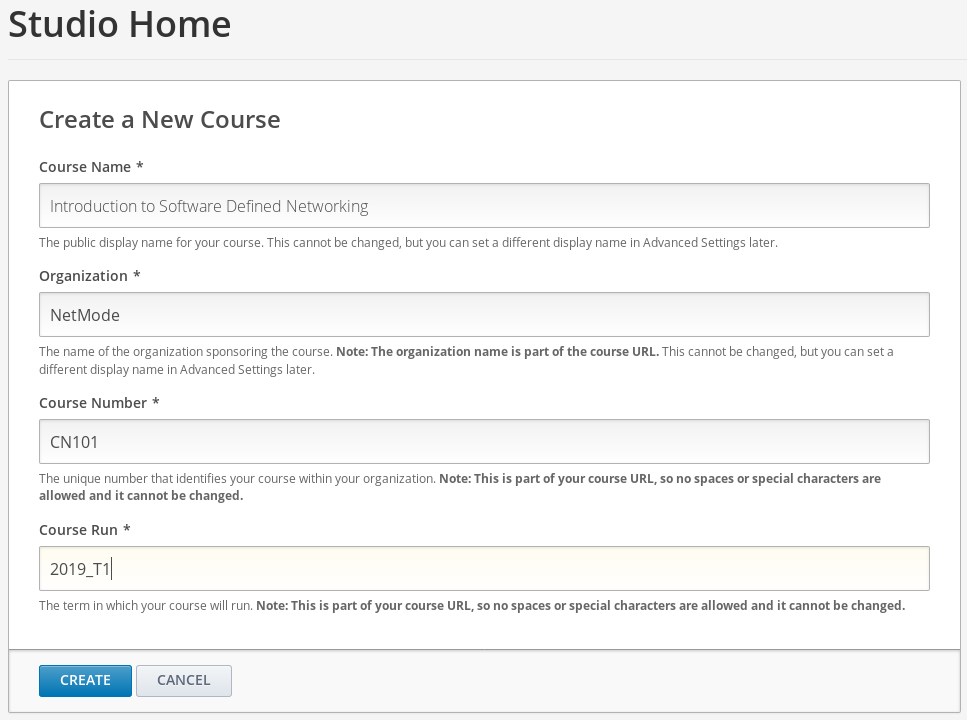
\includegraphics[width=0.8\textwidth, height=8cm]{edx-studio-new-course}
\caption{Σελίδα νέου Μαθήματος \textlatin{edX studio}}
\label{fig:edx-studio-new-course}
\end{figure}

Στη συνέχεια εφόσον δημιουργήσουμε το μάθημα μπορούμε να ορίσουμε διαδοχικά τις διδακτικές ενότητες και να προσθέσουμε το εκπαιδευτικό υλικό, όπως στην εικόνα~\ref{fig:edx-studio-course-outline}.
\begin{figure}[!htbp]
\centering
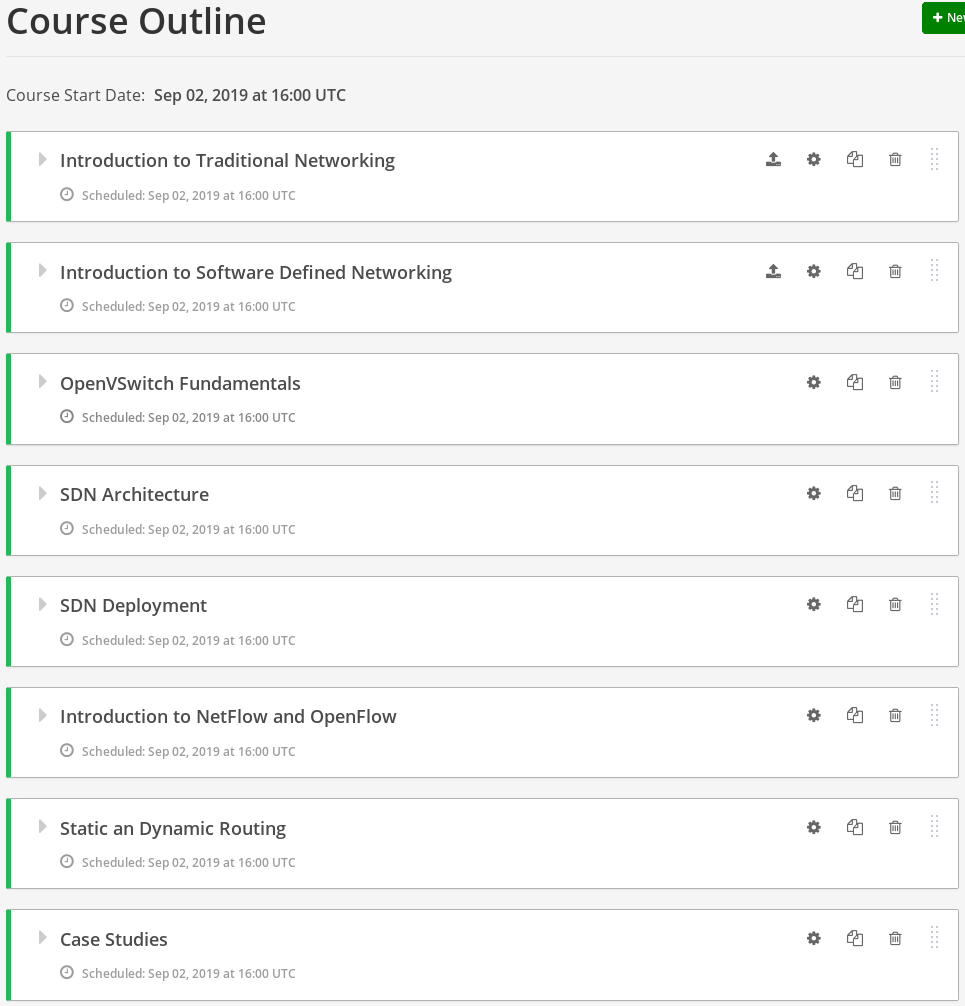
\includegraphics[width=0.8\textwidth, height=10cm]{edx-studio-course-outline}
\caption{Σελίδα προσθήκης νέου Εκπαιδευτικού Υλικού \textlatin{edX studio}}
\label{fig:edx-studio-course-outline}
\end{figure}

\section{Λειτουργικότητα Ιστοσελίδας}\label{lms_use}
\subsection{Αρχική Σελίδα}
Το πρώτο πράγμα που βλέπει κάποιος όταν επισκέπτεται την ιστοσελίδα είναι η φόρμα εισόδου. Ο κώδικας του \textlatin{microsite} παρέχει τη λειτουργικότητα της εισόδου υπαρχόντων (εικόνα~\ref{fig:microsite_login}) αλλα και της δημιουργίας νέων χρηστών της πλατφόρμας (εικόνα~\ref{fig:microsite_register}).

\begin{figure}[!htbp]
\centering
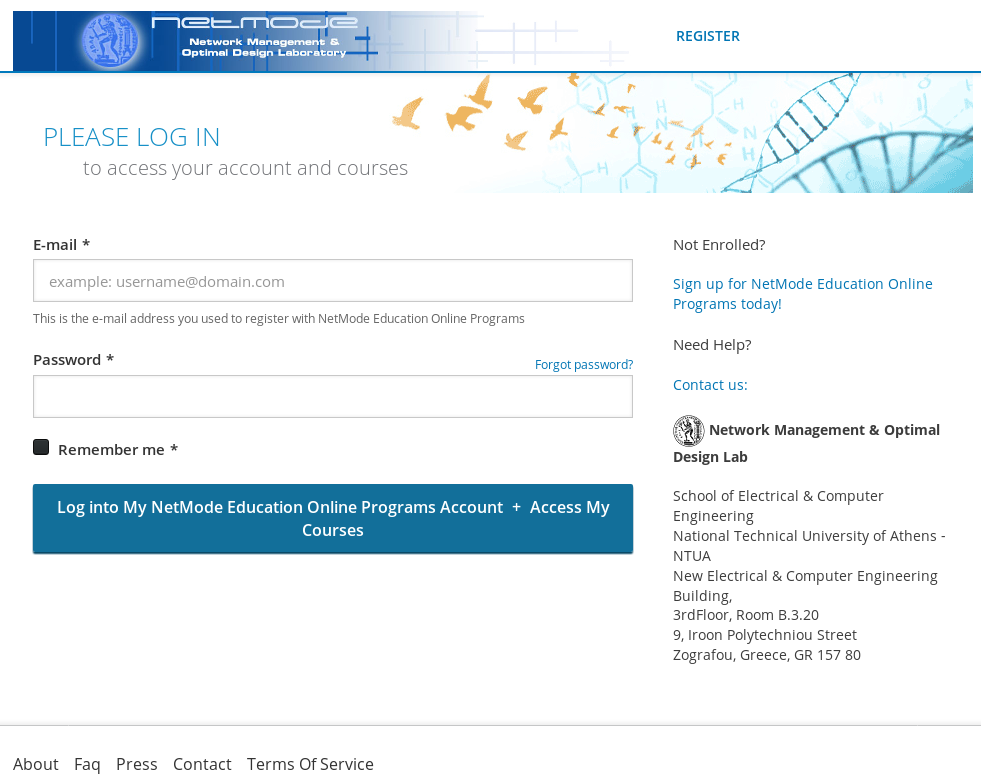
\includegraphics[width=0.8\textwidth, height=8cm]{microsite-login}
\caption{Σελίδα Εισόδου Χρηστών}
\label{fig:microsite_login}
\end{figure}

\begin{figure}[!htbp]
\centering
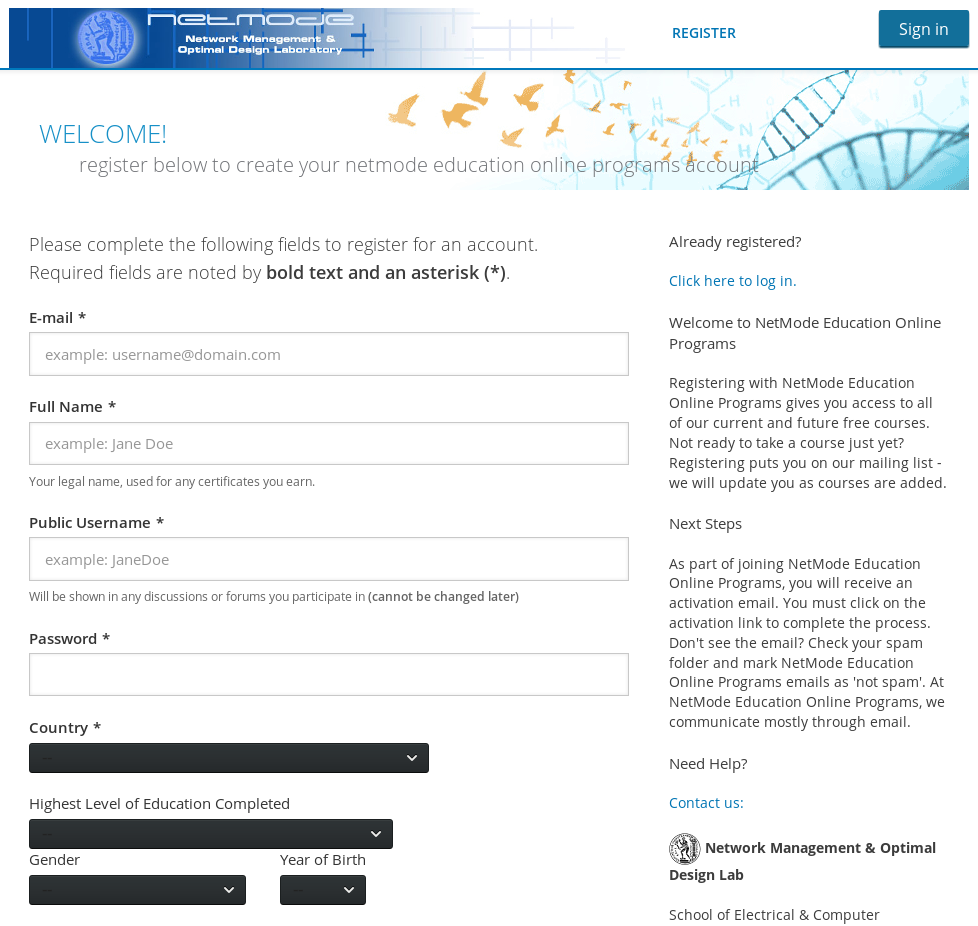
\includegraphics[width=0.8\textwidth, height=8cm]{microsite-register}
\caption{Σελίδα Εισαγωγής Νέου Χρήστη}
\label{fig:microsite_register}
\end{figure}

Μετά την είσοδο στην σελίδα παρουσιάζεται η αρχική σελίδα με τα διαθέσιμα μαθήματα, όπως στην εικόνα~\ref{fig:microsite-explore-course}. Για τις ανάγκες της εργασίας δημιουργήθηκε ένα ενδεικτικό μάθημα με τη χρήση του \textlatin{Studio}. Η διαδικασία δημιουργίας του μαθήματος περιγράφεται στο αντίστοιχο τμήμα~\ref{studio}.
\begin{figure}[!htbp]
\centering
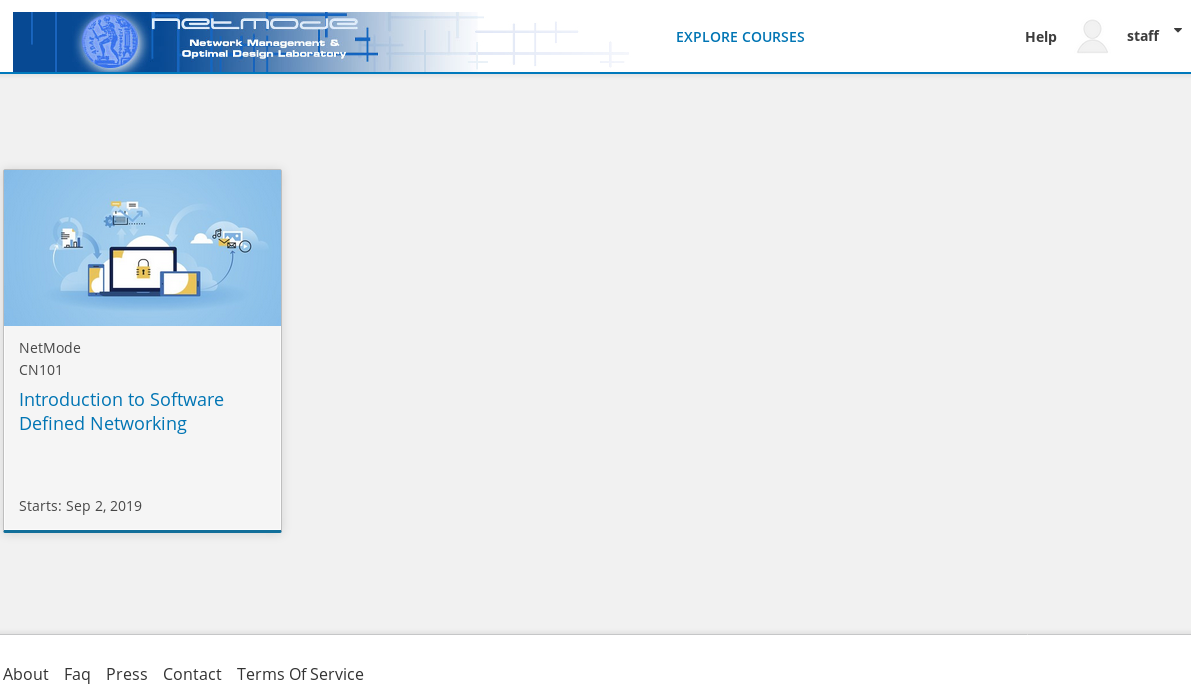
\includegraphics[width=0.8\textwidth, height=8cm]{microsite-explore-courses}
\caption{Σελίδα Πλοήγησης Μαθημάτων}
\label{fig:microsite-explore-course}
\end{figure}

\subsection{Επιλογή Μαθημάτων}
Μετά από την επιλογή ενός από τα διαθέσιμα μαθήματα, μεταφερόμαστε στην αντίστοιχη σελίδα (εικόνα~\ref{fig:microsite-course1}). Εκεί παρουσιάζεται συνοπτικά μια περιγραφή του μαθήματος, καθώς και διάφορα στοιχεία που αφορούν στην ημερομηνία έναρξης των παραδόσεων, τις ώρες εβδομαδιαίας διδασκαλίας, κ.α. Στη σελίδα αυτή υπάρχει η δυνατότητα ανάρτησης ενός εισαγωγικού βίντεο για την ενημέρωση των εκπαιδευομένων.
\begin{figure}[!htbp]
\centering
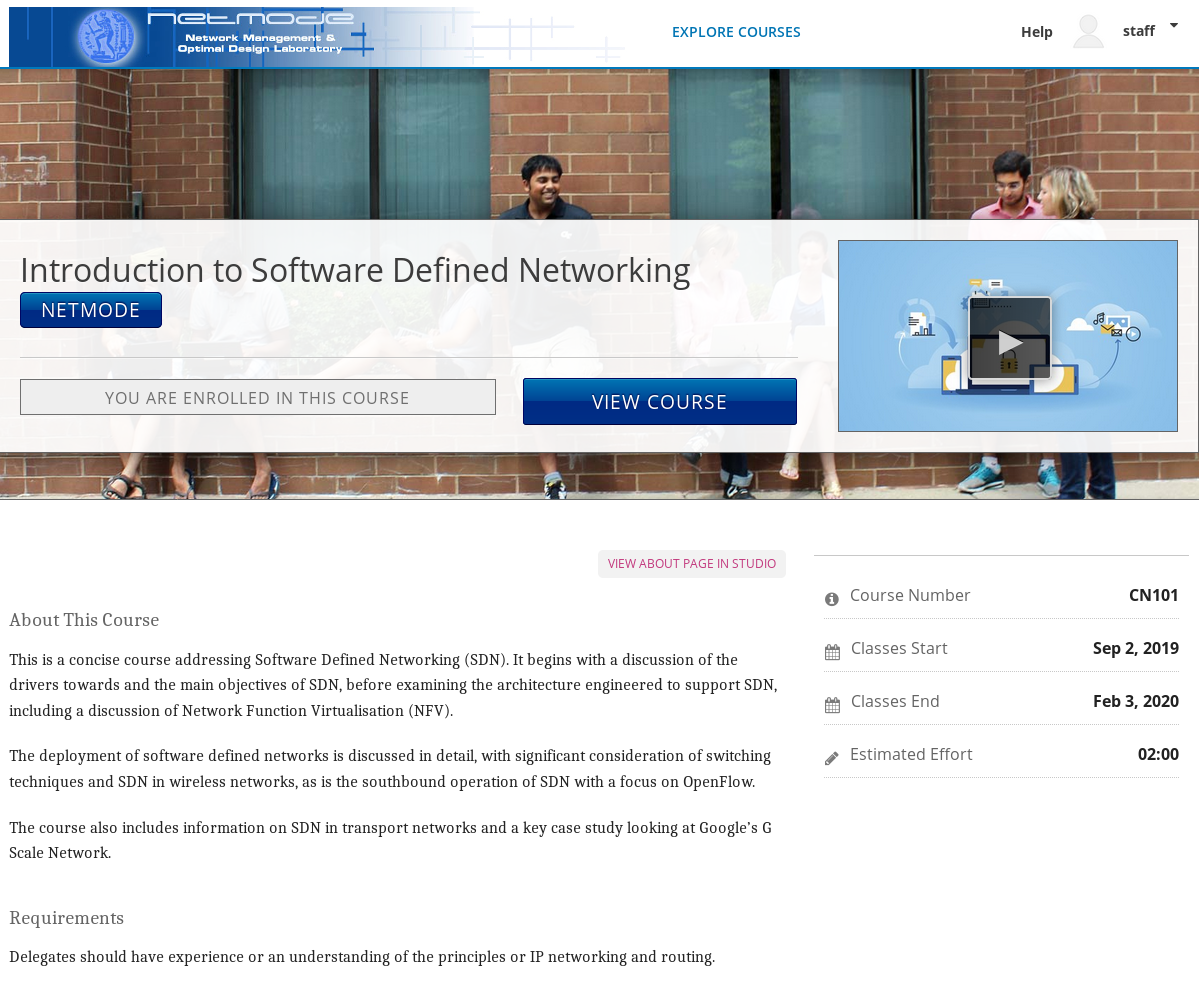
\includegraphics[width=0.8\textwidth, height=8cm]{microsite-course1}
\caption{Αρχική Σελίδα Μαθήματος}
\label{fig:microsite-course1}
\end{figure}

Η επιλογή \textlatin{"view course"} μας μεταφέρει σε μια συνοπτική περιγραφή των διδακτικών ενοτήτων, όπως αυτές καταχωρήθηκαν κατά την δημιουργία του μαθήματος στο \textlatin{studio} (τμήμα~\ref{studio} - εικόνα~\ref{fig:microsite-course2}). Από εδώ ο εκπαιδευόμενος μπορεί να επιλέξει μια από τις διαθέσιμες ενότητες, που τον ενδιαφέρει και πλοηγηθεί στο υλικό του μαθήματος (σημειώσεις, βιβλία, εκπαιδευτικά βίντεο, κτλ).
\begin{figure}[!htbp]
\centering
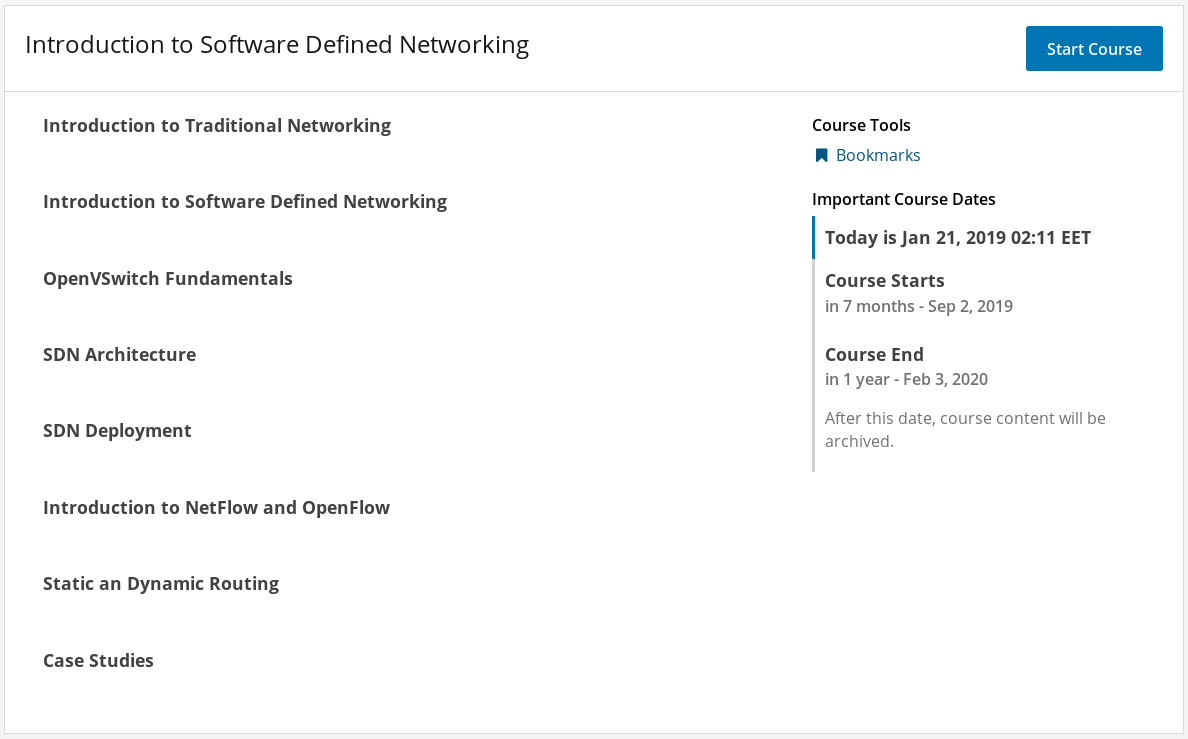
\includegraphics[width=0.8\textwidth, height=8cm]{microsite-course2}
\caption{Σελίδα Διδακτικών Ενοτήτων}
\label{fig:microsite-course2}
\end{figure}

\section{Συμπεράσματα}
Στο παρόν, παρουσιάστηκε συνοπτικά η διαδικασία εγκατάστασης της πλατφόρμας εξ' αποστάσεως εκπαίδευσης \textlatin{Open edX}, καθώς και η δημιουργία ενός ενδεικτικού μαθήματος με τη χρήση των αντίστοιχων εργαλείων. Αρχικά έγινε αναφορά σε βασικές έννοιες του ηλεκτρονικής μάθησης και της εξ' αποστάσεως εκπαίδευσης. Στη συνέχεια περιγράφηκαν τα εργαλεία τα οποία χρησιμοποιήθηκαν για την εγκατάσταση της πλατφόρμας \textlatin{edx} και ο τρόπος με τον οποίο αυτοματοποιήθηκαν και συνδυάστηκαν για την παραγωγή του τελικού αποτελέσματος, μετά και τη διαδικασία αποσφαλμάτωσης. Με τη βοήθεια των εργαλείων που προσφέρει η πλατφόρμα, δημιουργήθηκε ένα ενδεικτικό μάθημα, ενώ η διαδικασία αυτή παρουσιάστηκε με συνοπτικό τρόπο και τη βοήθεια ανάλογων \textlatin{screenshots}.

Το ηλεκτρονικό μάθημα της εργασίας παρέχει πλήρη λειτουργικότητα, η οποία είναι εύκολο να επεκταθεί με τη χρήση έτοιμων \textlatin{XBlocks} ή με σενάρια σε γλώσσα προγραμματισμού, όπως περιγράφηκε στο τμήμα~\ref{lms}.

\begin{appendices}
\chapter{Αρχείο Ρύθμισης Εικονικής Μηχανής \textlatin{Vagrantfile}}\label{AppA}
\selectlanguage{english}
\inputminted[linenos, fontsize=\scriptsize, breaklines, baselinestretch=1]{ruby}{sources/Vagrantfile}
\selectlanguage{greek}
\chapter{\textlatin{Bash Script} Εγκατάστασης \textlatin{Open edX}}\label{AppB}
\selectlanguage{english}
\inputminted[linenos, fontsize=\scriptsize, breaklines, baselinestretch=1]{bash}{sources/install_edx.sh}
\selectlanguage{greek}
\end{appendices}

\appendix

\bibliographystyle{babplain}
\bibliography{open-edx}

\end{document}